% Preamble
% ---
\documentclass{article}

% Packages
% ---
\usepackage{amsmath} % Advanced math typesetting
\usepackage[utf8]{inputenc} % Unicode support (Umlauts etc.)
\usepackage[ngerman]{babel} % Change hyphenation rules
\usepackage{hyperref} % Add a link to your document
\usepackage{graphicx} % Add pictures to your document
\usepackage{listings} % Source code formatting and highlighting

\begin{document}

\section{Prvi sloj i njegove parcijalne derivacije}

Ovdje su izvodi svih parcijalnih derivacija izlaza prvog sloja po parametrima. To će nam trebati kasnije kada ćemo izvoditi učenje svakog od parametara.

\begin{align*}
  & A_{i} = \frac{1}{1 + e^{b_{i}(x - a_{i})}} \\
  & \frac{\partial A_{i}}{\partial a_{i}} = \frac{1}{(1 + e^{b_{i}(x - a_{i})})^2} e^{b_{i}(x - a_{i})} b_{i} = A_{i}^{2} (\frac{1}{A_{i}} - 1) b_{i} = A_{i} (1 - A_{i}) b_{i} \\
  & \frac{\partial A_{i}}{\partial b_{i}} = \frac{-1}{(1 + e^{b_{i}(x - a_{i})})^2} e^{b_{i}(x - a_{i})} (x - a_{i}) = -A_{i}^{2} (\frac{1}{A_{i}} - 1) (x - a_{i}) = -A_{i}(1 - A_{i})(x - a_{i})
  \\ \\
  & B_{i} = \frac{1}{1 + e^{d_{i}(y - c_{i})}} \\
  & \frac{\partial B_{i}}{\partial c_{i}} = \frac{1}{(1 + e^{d_{i}(x - c_{i})})^2} e^{d_{i}(y - c_{i})} d_{i} = B_{i}^{2} (\frac{1}{B_{i}} - 1) d_{i} = B_{i} (1 - B_{i}) d_{i} \\
  & \frac{\partial B_{i}}{\partial d_{i}} = \frac{-1}{(1 + e^{d_{i}(x - c_{i})})^2} e^{d_{i}(y - c_{i})} (y - c_{i}) = -B_{i}^{2} (\frac{1}{B_{i}} - 1) (y - c_{i}) = -B_{i}(1 - B_{i})(y - c_{i})
\end{align*}

%\vspace{10mm}
\section{Drugi sloj i njegove parcijalne derivacije}

\begin{align*}
 	w_{i} =& A_{i} B_{i} \\ \\
	\frac{\partial w_{i}}{\partial A_{i}} = B_{i} \hspace{5mm} & \hspace{5mm} \frac{\partial w_{i}}{\partial B_{i}} = A_{i}
\end{align*}

%\vspace{10mm}
\section{Treći sloj i njegove parcijalne derivacije}
Ovaj sloj je normalizacijski sloj za kojeg neću posebno izvoditi derivacije, jer je lakše koristiti samo tu sumu kasnije u računu. Normalizacija svake od dobivenih težina provodi se na sljedeći način:


\begin{align*}
	\overline{w}_i = \frac{w_i}{\sum_{j=1}^{M} w_j}
\end{align*}

%\vspace{10mm}
\section{Četvrti i peti sloj i njihove parcijalne derivacije}
\begin{align*}
  f_{i} = p_{i} x + q_{i} y + r_{i} \\
  f = \frac{\sum_{i=1}^{M} w_{i}f_{i}}{\sum_{i=1}^{M} w_i}
\end{align*}
\begin{align*}
  &\frac{\partial f}{\partial f_i} = \frac{w_{i}}{\sum_{i=1}^{M} w_{i}} = \overline{w}_i \hspace{5mm} \hspace{5mm} \frac{\partial f}{\partial w_i} = \frac{f_{i} \sum_{j=1}^{M} w_{j} - \sum_{j=1}^{M} f_{j}w_{j}}{(\sum_{j=1}^{M} w_{j})^2} = \frac{\sum_{j=1}^{M} w_{j}(f_{i} - f_{j})}{(\sum_{j=1}^{M} w_{j})^2} \\ \\
  &\frac{\partial f_{i}}{\partial p_{i}} = x \hspace{1cm}
  \frac{\partial f_{i}}{\partial q_{i}} = y \hspace{1cm}
  \frac{\partial f_{i}}{\partial r_{i}} = 1 \\ \\
\end{align*}

%\vspace{10mm}
\section{Pogreška izlaza mreže}
$E$ je oznaka pogreške za $1$ podatak pri čemu je $y$ točna oznaka za podatak, a $f$ je izlaz mreže za taj isti podatak.

\begin{align*}
	E = \frac{1}{2}(y - f)^2 \\ \\
	\frac{\partial E}{\partial f} = -(y - f)
\end{align*}

\section{Određivanje pravila učenja za svaki od parametara}
Ideja je svaki od parametara (koji god da bio) mijenjati tako da se pomičemo u negativnom smjeru gradijenta pogreške $E$ po tom parametru za dani podatak. Za proizvoljan parametar $\theta$ to bi glasilo:

\begin{align*}
	\theta_{t+1} = \theta_{t} - \eta\frac{\partial E}{\partial \theta} 
\end{align*}

Budući da je gradijent (u ovom slučaju parcijalna derivacija) smjer najvećeg rasta funkcije, pomicanjem u negativnom smjeru gradijenta idemo u smjeru najvećeg pada ciljne funkcije (u ovom slučaju funkcije pogreške $E$) i to je ono što nam odgovara jer želimo minimizirati pogrešku. Hiperparametar $\eta$ je stopa učenja kojom reguliramo da koraci budu dovoljno maleni kako ne bi došlo do divergencije gradijentnog spusta.

% TODO:
%	sve one parcijalne derivacije
% 	dfi / dpi	dfi / dqi	dfi / dri
%	slike potrebne u izvjestaju

Odredimo sada parcijalne derivacije pogreške po svakom od parametara:

\begin{align*}
	&\frac{\partial E}{\partial a_{i}} = \frac{\partial E}{\partial f} \frac{\partial f}{\partial w_{i}} \frac{\partial w_{i}}{\partial A_{i}} \frac{\partial A_{i}}{\partial a_{i}} \hspace{5mm} & \hspace{5mm} \frac{\partial E}{\partial p_{i}} = \frac{\partial E}{\partial f} \frac{\partial f}{\partial f_{i}} \frac{\partial f_{i}}{\partial p_{i}} \\ \\
	&\frac{\partial E}{\partial b_{i}} = \frac{\partial E}{\partial f} \frac{\partial f}{\partial w_{i}} \frac{\partial w_{i}}{\partial A_{i}} \frac{\partial A_{i}}{\partial b_{i}} \hspace{5mm} & \hspace{5mm} \frac{\partial E}{\partial q_{i}} = \frac{\partial E}{\partial f} \frac{\partial f}{\partial f_{i}} \frac{\partial f_{i}}{\partial q_{i}} \\ \\
	&\frac{\partial E}{\partial c_{i}} = \frac{\partial E}{\partial f} \frac{\partial f}{\partial w_{i}} \frac{\partial w_{i}}{\partial B_{i}} \frac{\partial B_{i}}{\partial c_{i}} \hspace{5mm} & \hspace{5mm} \frac{\partial E}{\partial r_{i}} = \frac{\partial E}{\partial f} \frac{\partial f}{\partial f_{i}} \frac{\partial f_{i}}{\partial r_{i}} \\ \\
	&\frac{\partial E}{\partial d_{i}} = \frac{\partial E}{\partial f} \frac{\partial f}{\partial w_{i}} \frac{\partial w_{i}}{\partial B_{i}} \frac{\partial B_{i}}{\partial d_{i}} 
\end{align*}

Uvrštavanjem prije dobivenih izraza u svaku od jednadžbi dobivamo:

\begin{align*}
	&\frac{\partial E}{\partial a_{i}} = -(y - f) \frac{\sum_{j=1}^{M} w_{j}(f_{i} - f_{j})}{(\sum_{j=1}^{M} w_{j})^2} B_{i} A_{i} (1 - A_{i}) b_{i} \\ \\
	&\frac{\partial E}{\partial b_{i}} = -(y - f) \frac{\sum_{j=1}^{M} w_{j}(f_{i} - f_{j})}{(\sum_{j=1}^{M} w_{j})^2} B_{i} (-A_{i})(1 - A_{i})(x - a_{i}) \\ \\
	&\frac{\partial E}{\partial c_{i}} = -(y - f) \frac{\sum_{j=1}^{M} w_{j}(f_{i} - f_{j})}{(\sum_{j=1}^{M} w_{j})^2} A_{i} B_{i} (1 - B_{i}) d_{i} \\ \\
	&\frac{\partial E}{\partial d_{i}} = -(y - f) \frac{\sum_{j=1}^{M} w_{j}(f_{i} - f_{j})}{(\sum_{j=1}^{M} w_{j})^2} A_{i} (-B_{i})(1 - B_{i})(y - c_{i}) \\ \\
	&\frac{\partial E}{\partial p_{i}} = -(y - f) \frac{w_{i}}{\sum_{j=1}^{M} w_{j}} x \hspace{1cm}
	\frac{\partial E}{\partial q_{i}} = -(y - f) \frac{w_{i}}{\sum_{j=1}^{M} w_{j}} y \hspace{1cm}
	\frac{\partial E}{\partial r_{i}} = -(y - f) \frac{w_{i}}{\sum_{j=1}^{M} w_{j}} \\
\end{align*}


Prema pravilu učenja za proizvoljan parametar obnavljat ćemo vrijednosti svakog od parametara u algoritmu. Međutim javljaju se dvije inačice algoritma učenja: stohastička i grupna. Stohastička se inačica algoritma ponaša tako da obnavlja parametere nakon svakog podatka koji prođe kroz mrežu, pa se tako u jednoj epohi parameteri obnavljaju $N$ puta gdje je $N$ broj podataka za učenje. Grupa se pak inačica ponaša tako da uprosječuje gradijente po svim uzorcima za učenje i tako se parameteri obnavljaju samo jednom u jednoj epohi učenja. 

\section{Ciljna funkcija}

Ciljna funkcija glasi:
\begin{align*}
	((x - 1)^2 + (y + 2)^2 - 5xy + 3) * cos^2(\frac{x}{5})
\end{align*}

i njen izgled je prikazan na slici \ref{fig:function_f}

\begin{figure}
  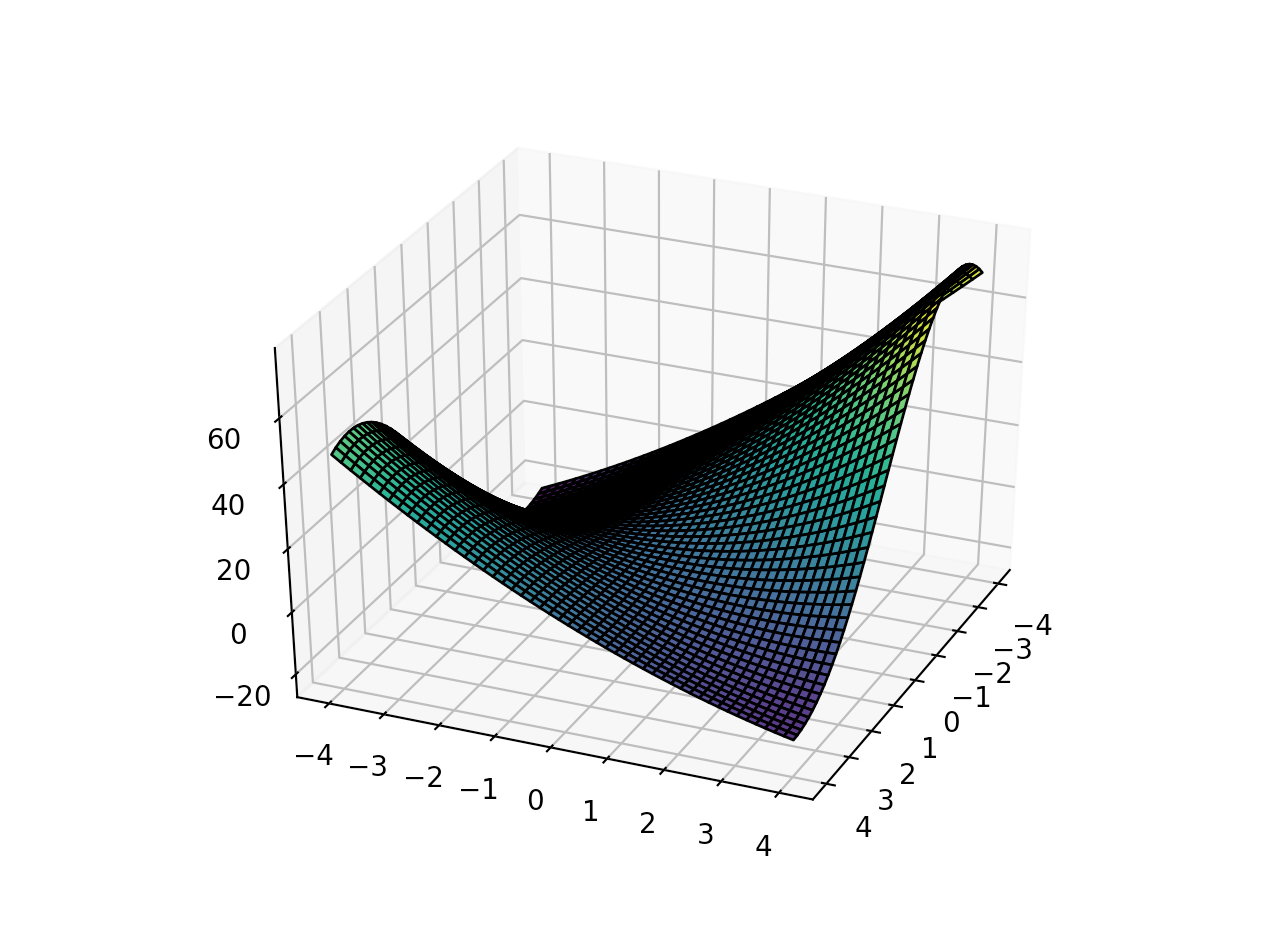
\includegraphics[width=\linewidth]{function_f.png}
  \caption{Ciljna funkcija} %x \in [-4, 4], y \in [-4, 4]}
  \label{fig:function_f}
\end{figure}


\section{Prikaz rada mreže za različiti broj pravila}

\begin{figure}
  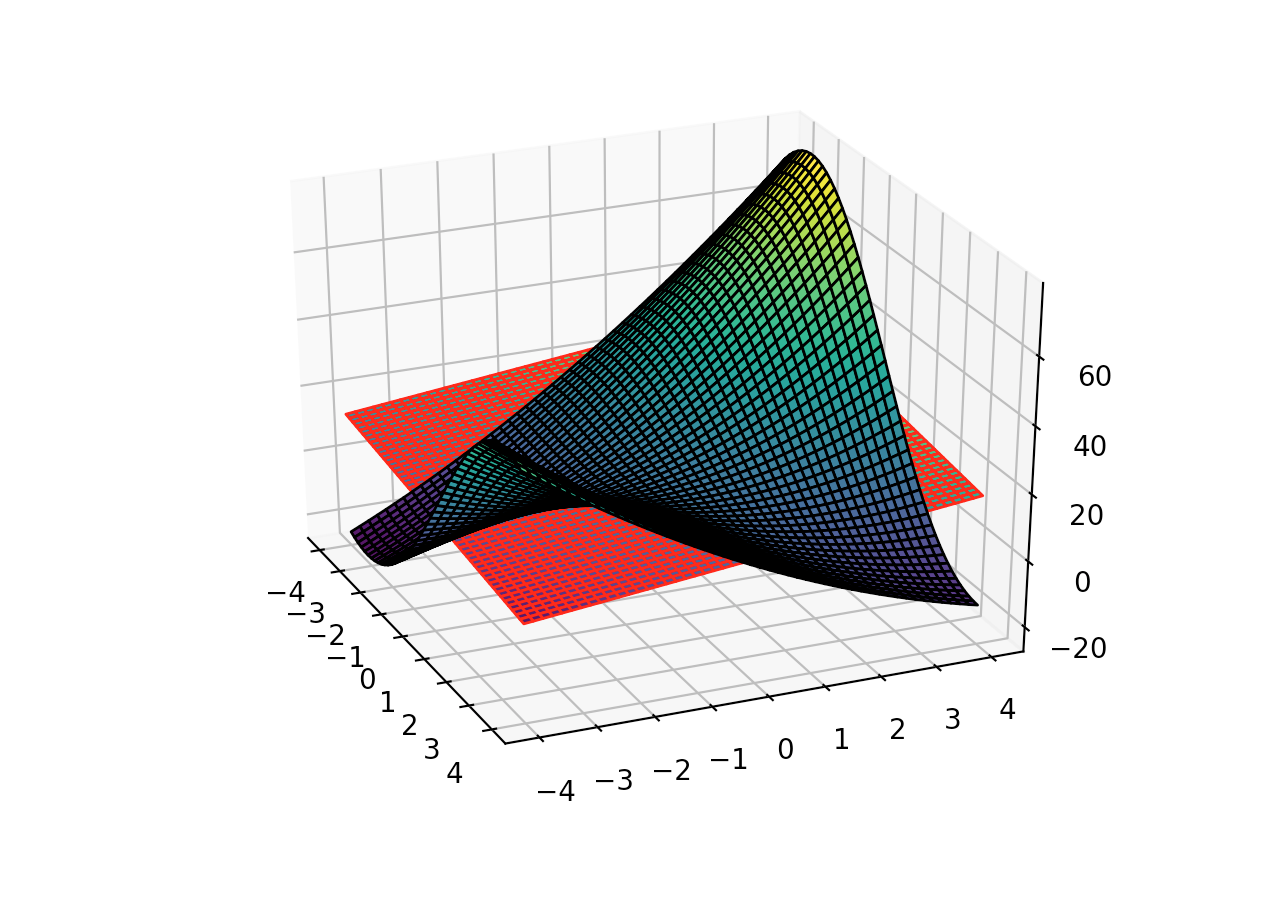
\includegraphics[width=\linewidth]{net1_plot.png}
  \caption{Izgled naučene funkcije za samo jedno pravilo.}
  \label{fig:net1_plot}
\end{figure}

\begin{figure}
  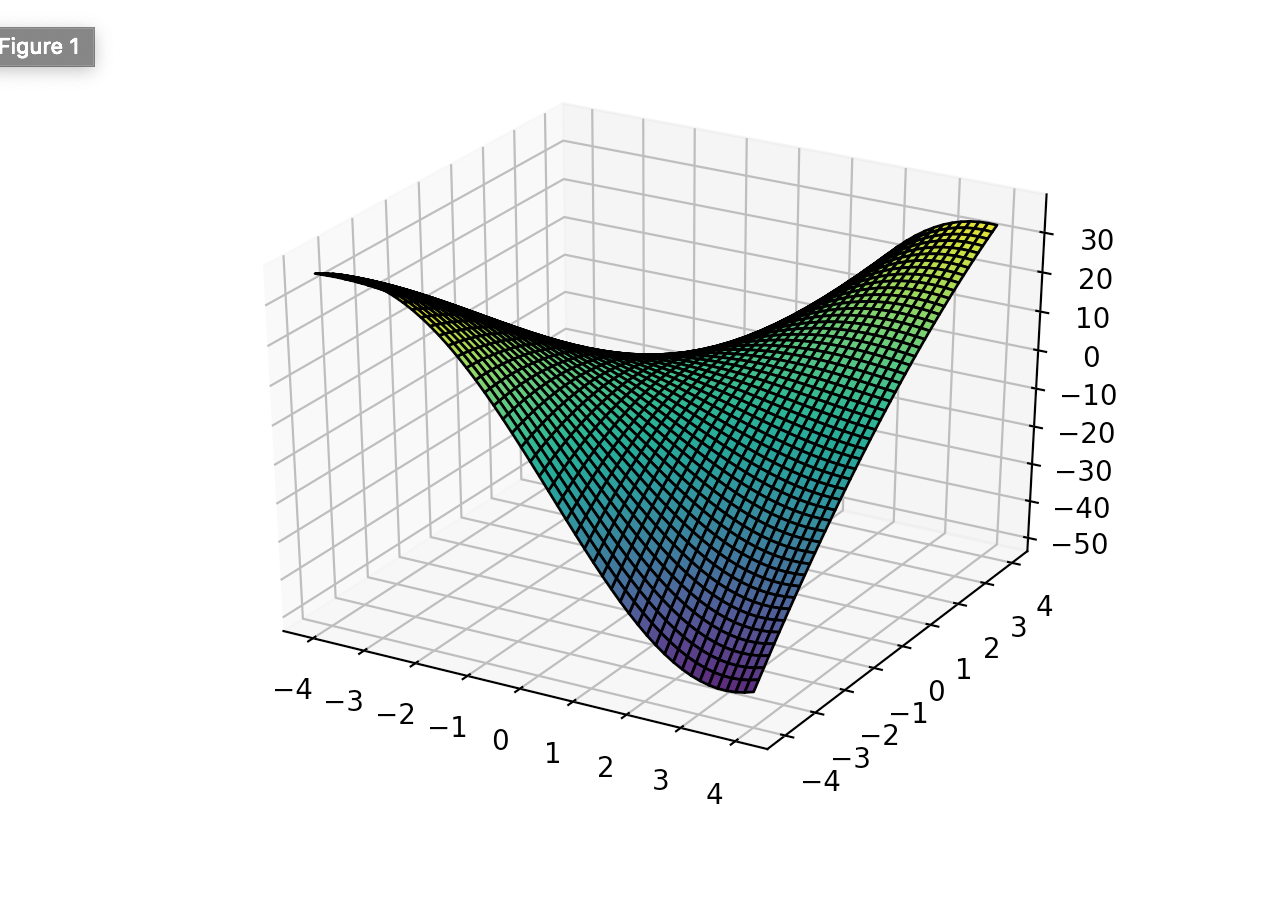
\includegraphics[width=\linewidth]{net1_error.png}
  \caption{Ploha pogreške za samo jedno pravilo.}
  \label{fig:net1_error}
\end{figure}

\begin{figure}
  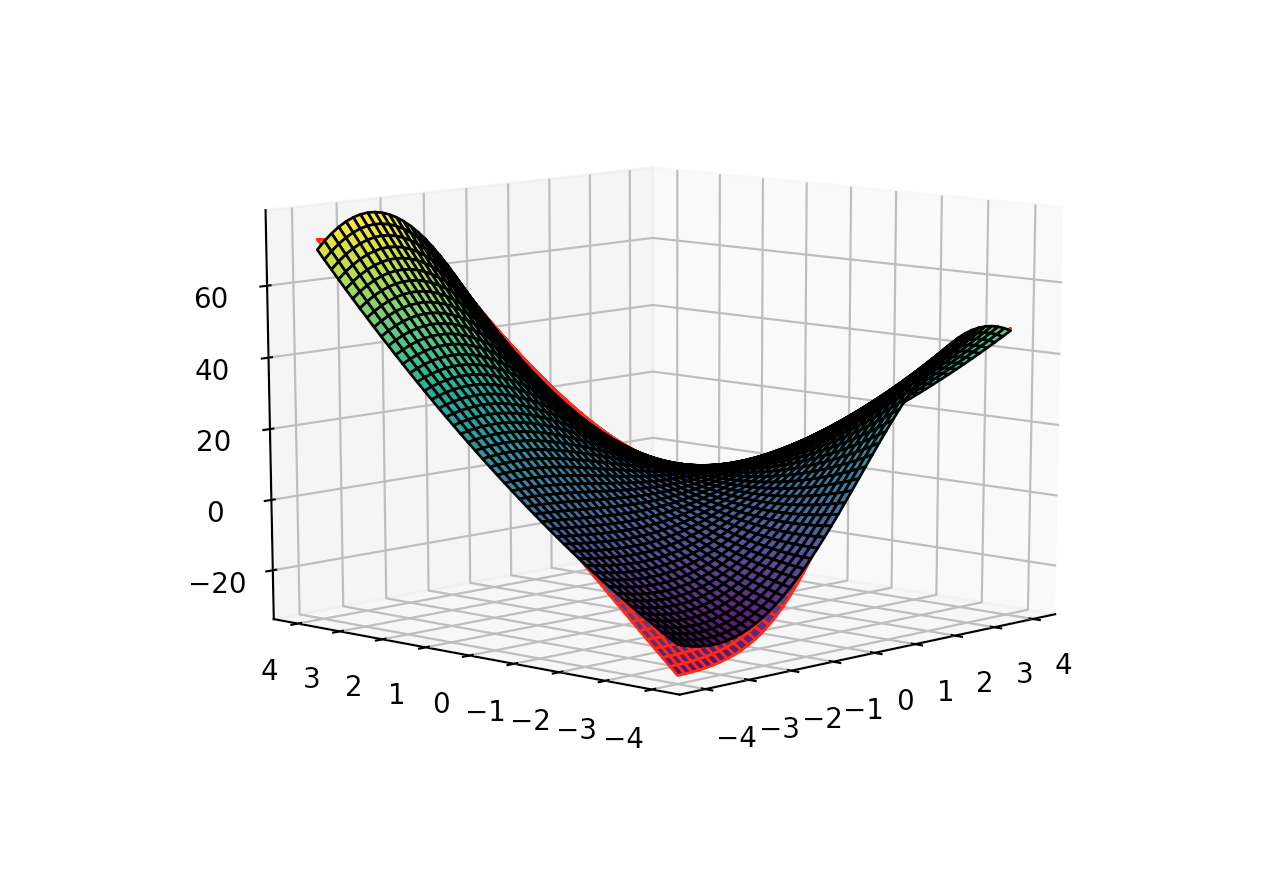
\includegraphics[width=\linewidth]{net2_plot.png}
  \caption{Izgled naučene funkcije za dva pravila.}
  \label{fig:net2_plot}
\end{figure}

\begin{figure}
  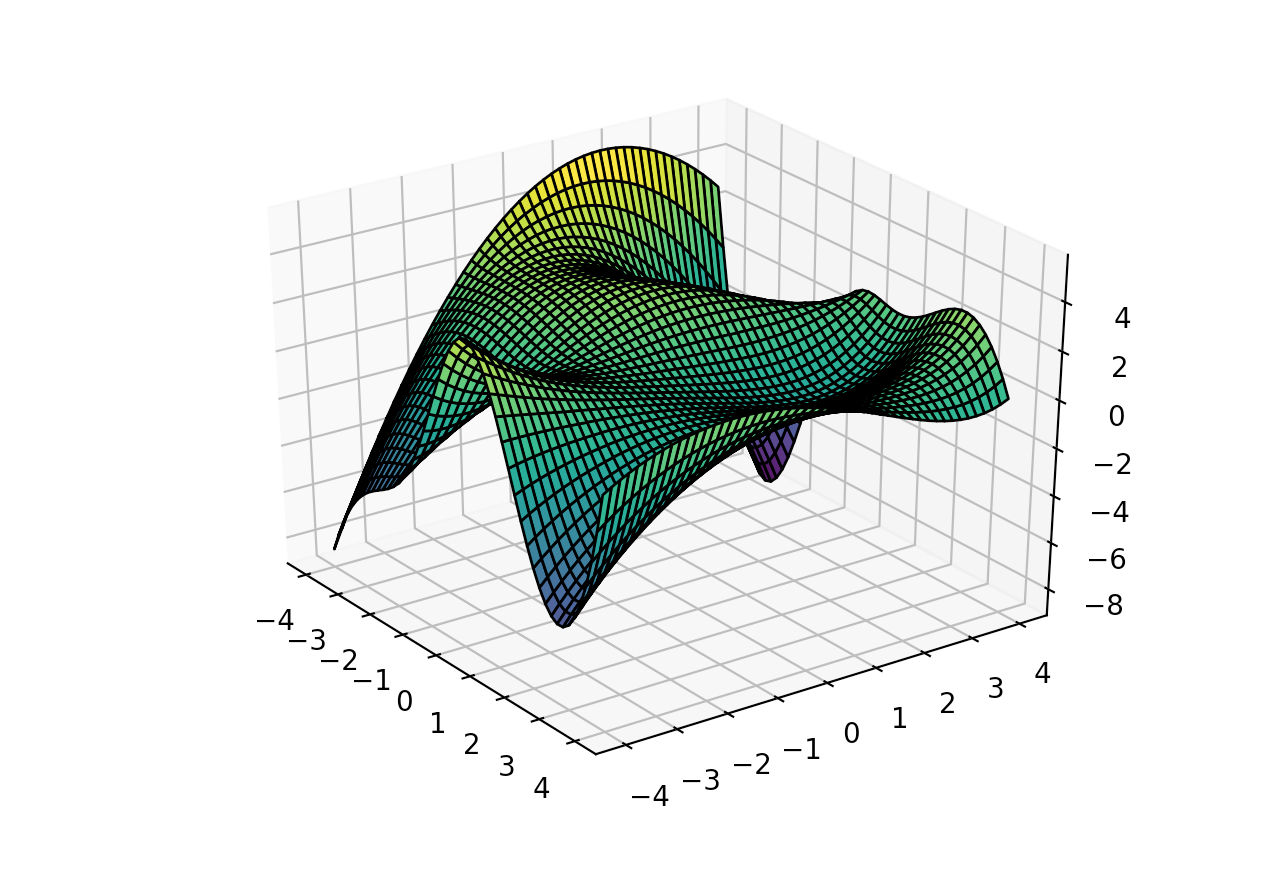
\includegraphics[width=\linewidth]{net2_error.png}
  \caption{Ploha pogreške za dva pravila.}
  \label{fig:net2_error}
\end{figure}

\begin{figure}
  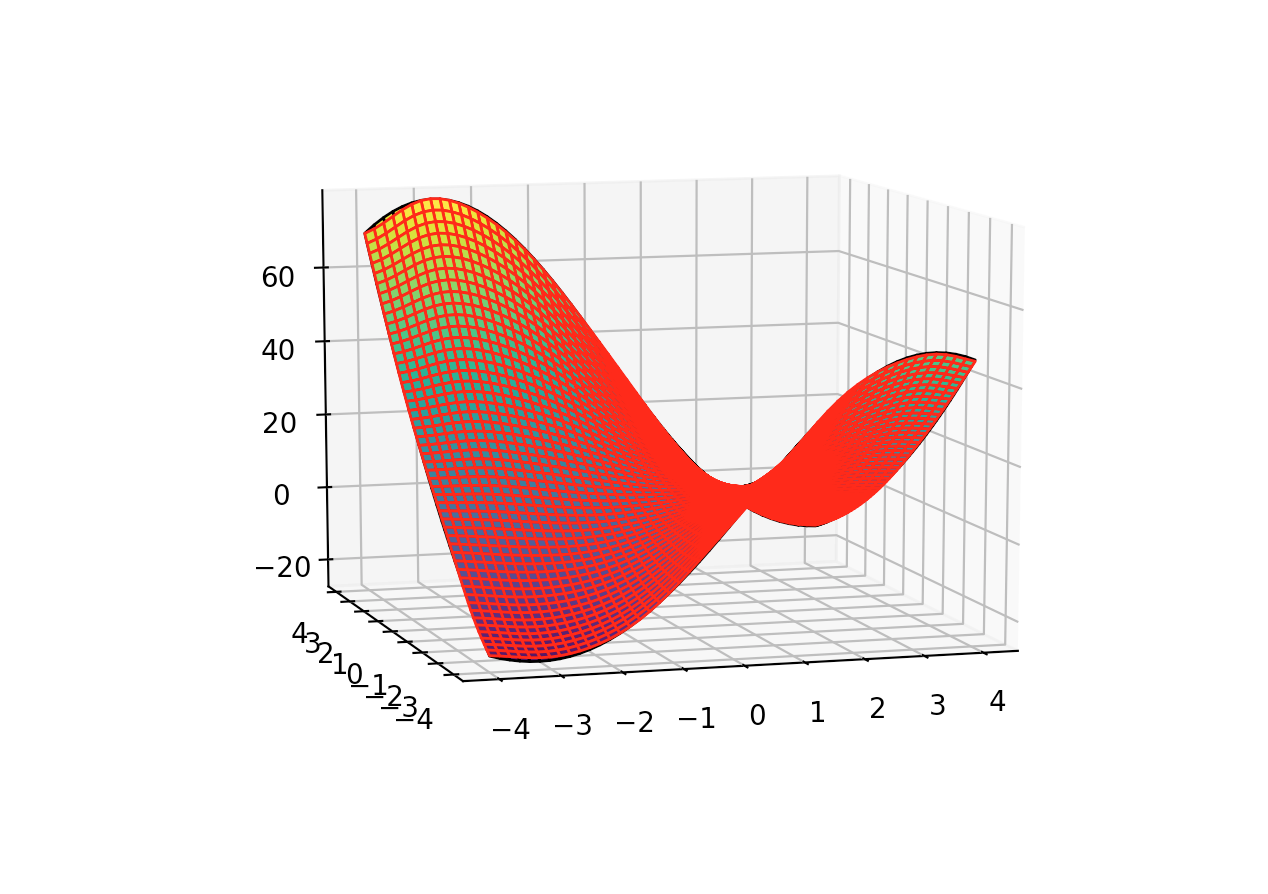
\includegraphics[width=\linewidth]{net8_plot.png}
  \caption{Izgled naučene funkcije za osam pravila.}
  \label{fig:net8_plot}
\end{figure}

\begin{figure}
  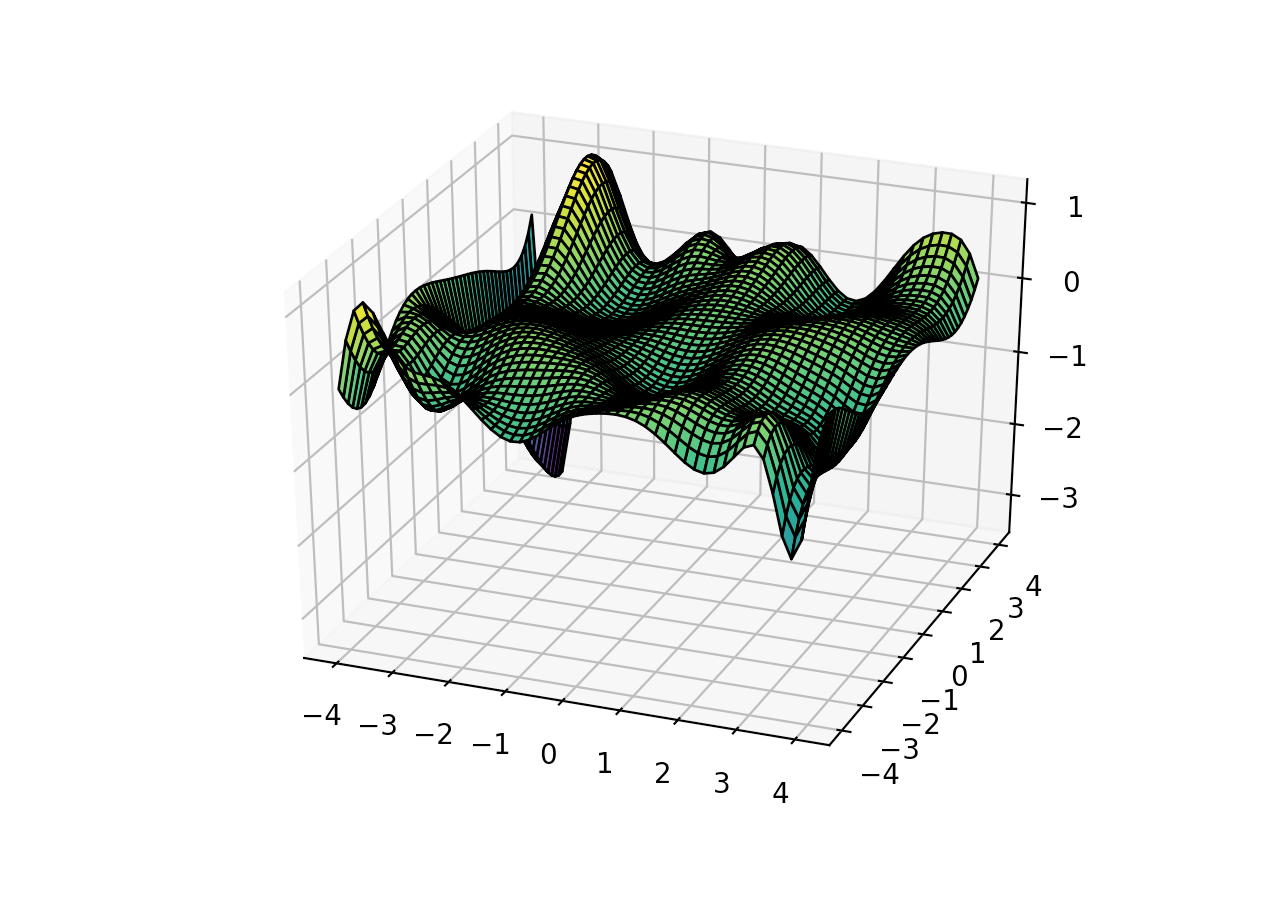
\includegraphics[width=\linewidth]{net8_error.png}
  \caption{Ploha pogreške za osam pravila.}
  \label{fig:net8_error}
\end{figure}

\begin{figure}
  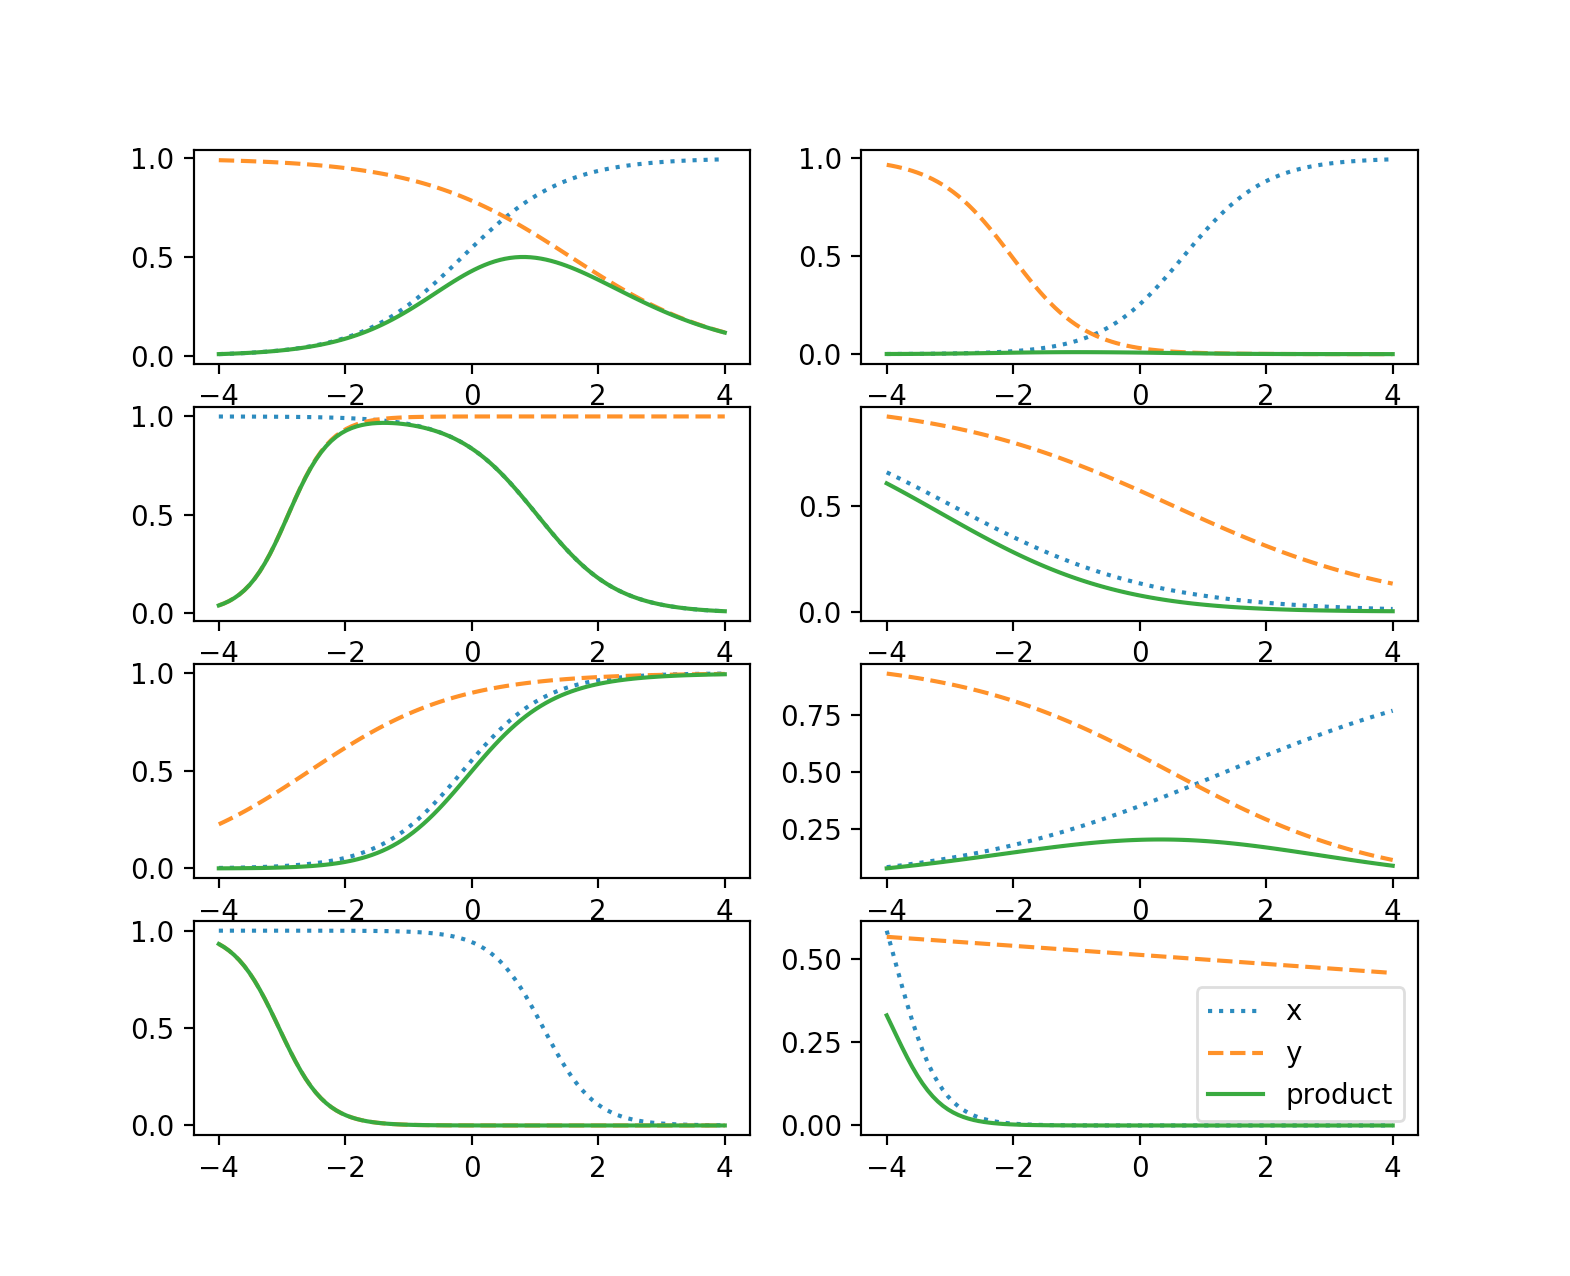
\includegraphics[width=\linewidth]{rules_8.png}
  \caption{Naučene funkcije pripadnosti za 8 pravila.}
  \label{fig:rules_8}
\end{figure}

\end{document}


